\subsection{Jacobian 判别法}

设 \(k\) 为环，A 为 \(k\)-代数，J 为 A 的理想，而 \(\bar{d}:\mathrm{J / J^{2}}\to A /\mathrm{J}\otimes_{\mathrm{A}}\Omega_{k}(\mathrm{A})\) 为典范映射。对每个 A/J-代数 R，我们用

\[
\bar {d} _ {\mathrm{R}}: \mathrm{R} \otimes_ {A / \mathrm{J}} \mathrm{J} / \mathrm{J} ^ {2} \longrightarrow \mathrm{R} \otimes_ {\mathrm{A}} \Omega_ {k} (\mathrm{A})
\]

表示由 \(\bar{d}\) 导出的 R-线性映射。若 k-代数 A/J 形式光滑，则 \(\bar{d}\) 具有 A-线性收缩（第 2 节，注 1），并且对每个 R，\(\bar{d}_{R}\) 都具有 R-线性收缩。

更一般地：

引理 3.—— 设 K 为 A 的一个包含 J 的理想。假设存在整数 m，使 \(J \cap K^{m}\) 含于 JK（当 A 为 Noether 环时此条件满足）。若 A/J 关于 K/J-进拓扑在 k 上形式光滑，则映射 \(\bar{d}_{A/K}: A/K \otimes_{A/J} J/J^{2} \longrightarrow A/K \otimes_{A} \Omega_{k}(A)\) 具有 A-线性收缩。

用 C 表示 \(k\)-代数 \(\mathrm{A} / (\mathrm{JK} + \mathrm{K}^m)\)；C 的理想 \(\mathrm{N} = (\mathrm{J} + \mathrm{K}^m) / (\mathrm{JK} + \mathrm{K}^m)\) 平方为零，且商环 C/N 与 \(\mathrm{A} / (\mathrm{J} + \mathrm{K}^m)\) 等同。给 C 与 C/N 赋以离散拓扑，给 A/J 赋以 K/J-进拓扑。典范同态 \(\mathrm{A} / \mathrm{J} \to \mathrm{A} / (\mathrm{J} + \mathrm{K}^m)\) 是连续的；因此它有一个提升 \(\varphi : \mathrm{A} / \mathrm{J} \to \mathrm{A} / (\mathrm{JK} + \mathrm{K}^m)\)。

于是，从 A 到 N 的映射 \(a \mapsto a1_{\mathrm{C}} - \varphi(a1_{\mathrm{A/J}})\) 是一个 \(k\)-导子（\(n^{\circ} 1\)，命题 1），故可写成 \(a \mapsto u(da)\)，其中 \(u \in \mathrm{Hom}_{\mathrm{A}}(\Omega_k(\mathrm{A}), \mathrm{N})\)。但假设 \(\mathrm{J} \cap \mathrm{K}^m \subset \mathrm{JK}\) 蕴含 \(\mathrm{J} \cap (\mathrm{JK} + \mathrm{K}^m) = \mathrm{JK}\)，故典范映射 \(\psi: \mathrm{J/JK} \to \mathrm{N}\) 是双射；因此存在 \(v \in \mathrm{Hom}_{\mathrm{A/K}}(\mathrm{A/K} \otimes_{\mathrm{A}} \Omega_k(\mathrm{A}), \mathrm{J/JK})\)，使得对 A 中的 a，有 \(a1_{\mathrm{C}} = \varphi(a1_{\mathrm{A/J}}) + \psi(v(1 \otimes da))\)。取 a 属于 J，即见 \(v(1 \otimes da)\) 等于 a 在 J/JK 中的类。由于 \(\mathrm{A/K} \otimes_{\mathrm{A/J}} \mathrm{J/J}^2\) 与 J/JK 等同，v 就是所求的收缩。

当代数 A 为 Noether 环时关于 K 的条件成立这一事实，由 III, § 3, 第 1 节，命题 1 的推论 2 可得。

引理 4.—— 假设 A 关于 J-进拓扑在 k 上形式光滑。为使 A/J 在 k 上形式光滑，必须且只须典范映射 \(\bar{d}\) 具有 A-线性收缩。

我们已经知道，若 A/J 在 k 上形式光滑，则映射 \(\bar{d}\) 具有 A-线性收缩（第 2 节，注 1）。反之，假设 \(\bar{d}\) 具有 A-线性收缩。设 \(\pi: A/J^{2} \to A/J\) 为典范满射；由第 1 节的命题 2，存在环同态 \(h: A/J \to A/J^{2}\) 使 \(\pi \circ h = 1_{A/J}\)。设 C 为一个 k-代数，N 为 C 的一个平方为零的理想，\(\rho: C \to C/N\) 为典范满射；给 C 与 C/N 赋以离散拓扑。设 \(u: A/J \to C/N\) 为 k-代数的连续同态。由于 A 关于 J-进拓扑在 k 上形式光滑，存在 k-代数同态 \(v: A \to C\) 使该图表交换

\pandocbounded{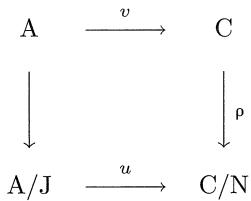
\includegraphics[keepaspectratio]{images/part001_bcdd9d30.jpg}}

其中竖直箭头表示典范满射。我们有 \(v(\mathrm{J})\subset\mathrm{N}\)，从而 \(v(\mathrm{J}^{2})\subset\mathrm{N}^{2}=\{0\}\)，于是 v 通过取商定义了一个同态 \(\bar{v}:\mathrm{A}/\mathrm{J}^{2}\to\mathrm{C}\)，它满足 \(\rho\circ\bar{v}=u\circ\pi\)。那么 \(\bar{v}\circ h\) 是 u 到 C 中的提升。

定理 3.—— 设 \(k\) 为环，A 为形式光滑的 \(k\)-代数，J 为 A 的有限生成理想；令 B=A/J。

\begin{enumerate}
\def\labelenumi{\alph{enumi})}
\tightlist
\item
  设 \(\mathfrak{p}\) 为 B 的素理想，\(\mathfrak{q}\) 为 A 中满足 \(\mathfrak{p}=\mathfrak{q}/J\) 的（素）理想。下列条件等价：
\end{enumerate}

\begin{enumerate}
\def\labelenumi{(\roman{enumi})}
\item
  k-代数 \(B_{\mathfrak{p}}\) 形式光滑；
\item
  存在 \(f\in B-\mathfrak{p}\) 使 k-代数 \(B_{f}\) 形式光滑；
\item
  \(\kappa (\mathfrak{p})\)-线性映射
\end{enumerate}

\[
\bar {d} _ {\kappa (\mathfrak {p})}: \kappa (\mathfrak {p}) \otimes_ {\mathrm{B}} \mathrm{J} / \mathrm{J} ^ {2} \rightarrow \kappa (\mathfrak {p}) \otimes_ {\mathrm{A}} \Omega_ {k} (\mathrm{A})
\]

是单射；

\begin{enumerate}
\def\labelenumi{(\roman{enumi})}
\setcounter{enumi}{3}
\tightlist
\item
  存在整数 \(m \geqslant 0\)、J 的元素 \(f_{1}, \ldots, f_{m}\)（其像 \((f_{1})_{\mathfrak{q}}, \ldots, (f_{m})_{\mathfrak{q}}\) 生成理想 \(J_{\mathfrak{q}}\)），以及 A 的 k-导子 \(D_{1}, \ldots, D_{m}\)，使 \(\det(\mathrm{D}_{j}(f_{i})) \not\in \mathfrak{q}\)。
\end{enumerate}

\begin{enumerate}
\def\labelenumi{\alph{enumi})}
\setcounter{enumi}{1}
\item
  B 中满足 (a) 的诸等价条件的素理想 p 组成的集合在 Spec(B) 中是开集。为使 B 在 k 上形式光滑，必须且只须 B 的每个素（相应地，极大）理想都满足这些条件。
\item
  假设 A 是 Noether 环。(a) 的条件也等价于：
\end{enumerate}

\begin{enumerate}
\def\labelenumi{(\alph{enumi})}
\setcounter{enumi}{21}
\tightlist
\item
  k-代数 \(B_{\mathfrak{p}}\) 关于 \(\mathfrak{p}B_{\mathfrak{p}}\)-进拓扑形式光滑。
\end{enumerate}

此外，在条件 (iv) 之下，理想 \(J_{\mathfrak{q}}\) 是完全割的，且序列 \(((f_{1})_{\mathfrak{q}},\ldots,(f_{m})_{\mathfrak{q}})\) 对 \(A_{\mathfrak{q}}\) 是完全割的。

令 \(M = J/J^{2}\)，\(N = B \otimes_{A} \Omega_{k}(A)\)。B-模 \(M\) 是有限型的，而 B-模 \(N\) 是投射的（\(n^{\circ} 5\)，定理 2 的推论 3）。对每个乘性子集 \(S\)（含于 \(A\)），\(k\)-代数 \(S^{-1}A\) 都形式光滑（\(n^{\circ} 2\)，命题 4, a)）。于是由引理 4，条件 (i) 与 (ii) 分别等价于

(i') 映射 \(\bar{d}_{B_{\mathfrak{p}}}:M_{\mathfrak{p}}\longrightarrow N_{\mathfrak{p}}\) 具有 \(B_{\mathfrak{p}}\)-线性收缩；

(ii') 存在 \(f \in \mathrm{B} - \mathfrak{p}\)，使映射 \(\tilde{d}_{\mathrm{B}_f}: \mathrm{M}_f \to \mathrm{N}_f\) 具有 \(\mathrm{B}_f\)-线性收缩。

把第 8 节的命题 9 应用于环 B 和同态 \(\bar{d}:M\to N\)，即得条件 (i')、(ii'') 与 (iii) 的等价性，并且（再次利用引理 4）也给出 (b) 中的断言。此外，(iii) 等价于：

(iii') 映射 \(\kappa(\mathfrak{q})\otimes_{\mathrm{A}}\mathrm{J}\longrightarrow\kappa(\mathfrak{q})\otimes_{\mathrm{A}}\Omega_{k}(\mathrm{A})\)（由 \(d:\mathrm{J}\to\Omega_{k}(\mathrm{A})\) 导出）是单射，

而 (iv) 可写成：

(iv') 存在整数 \(m\geqslant 0\)、J 的元素 \(f_{1},\ldots,f_{m}\)（其像生成理想 \(J_{\mathfrak{q}}\)，在环 \(A_{\mathfrak{q}}\) 中），以及元素 \(y_{1},\ldots,y_{m}\)（属于 \(\operatorname{Hom}_{\mathrm{A}}(\Omega_{k}(A),A)\)），使 \(\det(\langle y_{j},df_{i}\rangle)\notin\mathfrak{q}\)。

由于 \(\mathrm{A}\)-模 \(\Omega_{k}(A)\) 是投射的（第 5 节，定理 2 的推论 3），把第 8 节的命题 9 应用于环 A 和同态 \(d:\mathrm{J}\to\Omega_{k}(A)\)，即得 (iii') 与 (iv') 的等价性。

最后，假设环 A 是 Noether 环。显然 (i) 蕴含 (v)。在假设 (v) 之下，引理 3 表明映射

\[
\bar {d} _ {\kappa (\mathfrak {q})}: \kappa (\mathfrak {q}) \otimes_ {\mathrm{B} _ {\mathfrak {p}}} \mathrm{J} _ {\mathfrak {q}} / \mathrm{J} _ {\mathfrak {q}} ^ {2} \longrightarrow \kappa (\mathfrak {q}) \otimes_ {\mathrm{A} _ {\mathfrak {q}}} \Omega_ {k} (\mathrm{A} _ {\mathfrak {q}})
\]

是单射，从而得到 (iii)。

在条件 (iv) 之下，我们有 \(m=[\kappa(\mathfrak{q})\otimes_{\mathrm{A}}\mathrm{J}:\kappa(\mathfrak{q})]\)（第 9 节，命题 8）。根据第 5 节的定理 2，理想 \(J_{\mathfrak{q}}\) 是完全割的，且序列 \(((f_1)_{\mathfrak{q}},\ldots,(f_m)_{\mathfrak{q}})\) 对 \(A_{\mathfrak{q}}\) 是完全割的（§ 1, 第 3 节，定理 1 的推论 2）。这就证明了 c)。

推论 1.—— 设 \(k_{0}\) 为环，\(k\) 为 Noether 的形式光滑 \(k_{0}\)-代数，B 为本质有限型的局部 \(k\)-代数。若 \(k_{0}\)-代数 B 关于 \(\mathfrak{m}_{\mathrm{B}}\)-进拓扑形式光滑，则它形式光滑。

存在整数 \(n\geqslant 0\)、\(k[\mathrm{T}_{1},\ldots,\mathrm{T}_{n}]\) 的乘性子集 S，以及一个满的 \(k\)-同态 \(\mathrm{S}^{-1}k[\mathrm{T}_{1},\ldots,\mathrm{T}_{n}]\to\mathrm{B}\)。代数 \(\mathrm{S}^{-1}k[\mathrm{T}_{1},\ldots,\mathrm{T}_{n}]\) 是 Noether 的，且在 k 上形式光滑（第 3 节，例 2 及第 2 节，命题 4, a)），故在 \(k_{0}\) 上也形式光滑（第 2 节，命题 3, a)）。于是推论由定理 3, c) 得出。

推论 2.—— 设 \(k_{0}\) 为环，\(k\) 为 Noether 的形式光滑 \(k_{0}\)-代数，B 为本质有限型的 k-代数。由 B 中使 \(k_{0}\)-代数 \(B_{\mathfrak{p}}\) 形式光滑（关于离散拓扑或 \(\mathfrak{p}B_{\mathfrak{p}}\)-进拓扑）的素理想 p 组成的集合 U 在 Spec(B) 中是开集，且下列条件等价：

\begin{enumerate}
\def\labelenumi{(\roman{enumi})}
\item
  我们有 U = Spec(B)；
\item
  U 包含 B 的所有极大理想；
\item
  \(k_{0}\)-代数 B 形式光滑。
\end{enumerate}

这与前面一样由定理 3 得出。

注 1.—— 当 \(k_{0}\) 是域且我们处于下列两种情形之一时，推论 1 与 2 特别适用：

\begin{enumerate}
\def\labelenumi{\alph{enumi})}
\item
  B 是 \(k_{0}\) 的一个可分扩张上的本质有限型代数（第 3 节，定理 1）；
\item
  B 是 \(k_{0}\)-完备 Noether 局部代数，其剩余域 \(\kappa_{B}\) 是 \(k_{0}\) 的可分扩张（此时我们取 k 为 \(\kappa_{B}\) 上的一个形式幂级数代数，而 B 是它的一个商（第 3 节及 IX, § 3, 第 3 节））。
\end{enumerate}

在上述每种情形中，由推论 2，并考虑到第 7 节的命题 8 以及 § 6 第 4 节的命题 6, b)，可知 \(k_0\)-代数 B 形式光滑当且仅当它绝对正则。

推论 3 (Zariski)。设 \(k\) 为域，A 为正则的 \(k\)-局部代数，J 为 A 的一个不等于 A 的理想。我们假设 \(k\)-代数 A 是本质有限型的或完备的。为使局部环 A/J 正则，必须且只须存在整数 \(m \geqslant 0\)、生成 J 的 J 中元素 \(f_1, \ldots, f_m\)，以及 A 的导子 D \(_1, \ldots, D_m\)，使 det(D \(_j(f_i)\) ) \(\not\in \mathfrak{m}_{\mathrm{A}}\)。此时元素 (f \(_1, \ldots, f_m\) ) 构成 A 的一个坐标系的一部分，且理想 J 是素理想。

设 \(k_0\) 为 \(k\) 的素域。\(k_0\)-代数 A 绝对正则（§ 6, 第 4 节，例 1），故形式光滑（前面的注 1）。基于同样的理由，说 A/J 正则等价于说它是形式光滑的 \(k_0\)-代数。于是第一个断言由定理 3 得出，而定理 3 还蕴含序列 \((f_1,\ldots,f_m)\) 对 A 是完全割的。然后应用 VIII, § 5, 第 3 节的命题 2。

注 2.—— 在推论 3 的假设之下，A-模 \(\Omega(A)\) 是投射的（第 5 节，定理 2 的推论 3），故是自由的；于是 A 到 \(\kappa_{A}\) 中的每个导子都可提升为 A 的导子。因此命题中的条件可表述如下：存在 J 的生成系 \((f_{1},\ldots,f_{m})\) 与导子 \(D_{1},\ldots,D_{m}\)（从 A 到 \(\kappa_{A}\) 中），使 \(\det(D_{j}(f_{i}))\neq0\)。

推论 4 (Zariski)。—— 设 k 为域，A 为本质有限型的 k-代数或完备 Noether 局部环。由 A 中使局部环 A \(_{p}\) 正则的素理想 p 组成的集合在 Spec(A) 中是开集。

只需应用注 1，取 \(k_0\) 为 \(k\) 的素域即可。

